\chapter{System design}

In this chapter the previously collected information are used to design the system in detail.
The decision making process for that is documented here as well.

\section{Environment}

The environment of where the systems shall be deployed onto must be known for detailed design decisions, which will be elaborated here.

All Winslow instances are supposed to run inside a Docker container (as requested in \autoref{workflow:desired:docker}).
The host will be a Ubuntu or Debian Linux Servers with some having multiple Nvidia graphics cards.
There will be no graphical user interface available on these servers.

%\todo{env: shall be executed on ubuntu/debian linux servers, Docker}

\section{Storage Technology}

Storing and accessing data is one of the main concerns for Winslow.
In almost all use cases, there will be multiple Winslow instances that need to access the storage.
Because of that, it must be accessible from remote and from multiple Winslow instances simultaneously.
For that, the following technologies are reviewed: NFS or SMB/CIFS (\autoref{analysis:storage:organisation}),  GlusterFS (\autoref{glusterfs}), SeaweedFS (\autoref{seaweedfs}), OpenIO (\autoref{openio}), dCache (\autoref{dcache}) and HadoopFS (\autoref{hadoopfs}).

The following criteria were used for comparison, with a scoring system with points from 0 to 3, in which 0 means the best solution and 3 the worst - the lower the overall score the better:

\begin{itemize}
\item \textbf{Installation Overhead}:
How hard and extensive is the installation?
Is there a good documentation?
Is the package provided from within the main repository of Ubuntu, or alternatively, does it provide any other form of easy installation?
Scoring 0 for installation through the main repository, 1 for an external repository, 2 for distribution specific archive, 3 for any other installation.

\item \textbf{Dependencies}:
Are further services required for operation? 
How hard are they to setup?
Do they need any additional configuration?
Scoring 0 for no further dependencies, 1 for dependencies but without the need of configuration,  2 for dependencies that require manual configuration, 3 for dependencies that need to be installed manually and require manual configuration.

\item \textbf{Single Point of Failure}:
Is the solution decentralized and is it failure resilient?
Is it site- or rack-aware or provide replication mechanisms to compensate?
Scoring 0 for completely decentralized, 1 for decentralized but with dependency on centralized backend, 2 for mostly centralized but with load balancing approaches, 3 for no single point of failure mitigations.

\item \textbf{Docker integration}:
How easy is it to integrate with Docker?
Scoring 0 for native support, 1 for native but non-trivial support, 2 for support through additional exports facility, 3 for non-trivial solution.

\item \textbf{Failure concerns}:
Are there any noteworthy concerns?
Was an early local test successful and reliable?
Is it a known technology or \enquote{proven in use}?
Who is developing it and what are the support guarantees?
Scoring 0 for commonly used and no concerns, 1 for minor concerns, 2 for major uncertainty, 3 for abandoned technology.
\end{itemize}

In \autoref{comparision:storage} the results are displayed:

\begin{table}[H]
	\begin{tabular}{l|c|c|c|c|c|c|c}
				& NFS S.& SMB/CIFS S.& GlusterFS & SeaweedFs	& dCache 	& HDFS \\
		\hline
		Inst. 	& 0 	& 1 		& 0 		& 2 		& 3			& 1 \\
		Dep. 	& 1 	& 0			& 0 		& 0 		& 3 		& 1 \\
		SPoF 	& 2		& 3			& 0			& 2 		& 0			& 0 \\
		Docker 	& 0 	& 2 		& 2 		& 3 		& 2 		& 3 \\
		Fail.	& 0		& 0			& 1			& 2			& 2			& 0 \\
		\hline
		Score 	& 3		& 6			& 3			& 9			& 10		& 5 \\
	\end{tabular}
	\caption{Comparison of storage technologies}
	\label{comparision:storage}
\end{table}

The worst scoring tool in this comparison is dCache.
The installation overhead, missing documentation and uncertainty on reliable operation is too high for this project (see \autoref{dcache}).

For similar reasons SeaweedFs is placed second worst.
Local tests could not access SeaweedFs reliable when a node failed and there is no trivial support for Docker nor does it provide an NFS export.
Using it from within Docker would require each container to be manipulated so that the first operation is mounting the storage with a custom binary and through a FUSE\footnote{Filesystem in Userspace} mount.
The tool also seems to be developed by a single person which introduces further uncertainty about reliability and support in the future.

HDFS and SMB/CIFS seem to be no terrible choice, but no especially good one either in this use case.

The two best scoring storage solutions are a simple NFS share and GlusterFS.
While GlusterFS provides replication and decentralized access, a NFS share scores with its simplicity.
The idea is to start with a plain NFS share for Winslow which can natively be utilized by Docker as volume mount and to revisit later whether the need for replication and decentralization persists.
Because of the NFS interface export of GlusterFS, Winslow could then easily switch to GlusterFS by accessing the NFS export closest to its' instance.

\section{Event Synchronization and Communication}


kafka does what? persist events and provides them in an order(?), cant Winslow do this itself, so that no further dependency is required?

\todo{.}
https://docs.microsoft.com/de-de/azure/architecture/microservices/design/interservice-communication


raw TCP (how to connect, centralized? star? tree?) centralized works towards -> centralized master node
broadcast?
microservice REST
event bus? kafka
messaging queue mqtt
NFS provides filesystem, filesystems are kind of standardized

https://kafka.apache.org/protocol
\todo{.}


As discovered in \autoref{analysis:layer_2} there is a need for an event synchronization across Winslow instances.
Without proper coordination, race conditions could cause stages to be started multiple times simultaneously, corrupt workspaces, configuration or project files.
While starting too many stage executions are only wasting resources, data corruptions can lead to unrecoverable damage.

There are multiple ways to exchange data between systems that do not share the same process or machine.
The most flexible implementation can be achieved by implementing a custom protocol on a raw TCP socket which allows to exchange blobs\footnote{\todo{Binary Large Objects}} between exactly two nodes.
For a blob or message to reach all nodes, a connection to every other node, a centralized broker, another topology such as a tree structure or broadcast messages would be required.
Because this in itself seemed to be a complex subject, third party alternatives were investigated.

Apache Kafka \todo{CITE} is one such alternatives.
It is open source, distributed and is focused on data and event streams.
But it as every third party service, it introduces a dependency on the project.
Not only in regards to interfacing and driver implementation, but also for maintenance and setup.
Each Winslow Image would require to be shipped with a pre-configured Kafka service and the administrator must ensure that these services can reach each other - in addition to storage solution.

This was, where the idea appeared: Is it possible to not introduce any further dependencies to the system, but re-use the existing storage solution for synchronization and communication?
To answer this, one must first investigate the smallest building block required for synchronized communication.
Taking the idea from Kafka, an event stream, where the messages have are globally ordered: is it enough to provide synchronization over messages occurring in a synchronized sequence?

\todo{ACID in fundamentals?}
ACID, which stands for Atomicity, Consistency, Isolation and Durability, describes the needs a database must fulfill so that it does not suffer from side effects or data corruption when executing queries.
A series of changes might not be allowed to be intercepted (atomicity), must see and result in consistent data, is not allowed to interfere with simultaneously executed queries and guarantees that once completed successfully, is in fact persistent and will not be lost (durability).

\todo{filesystem is close}

\todo{DB principles: ACID}

\todo{...}

\todo{requires common a way to exchange messages}

\todo{all messages - called events - are published to all nodes}

\todo{using file system as bus}

\todo{clear and globally same order of events}

\todo{events consist of an id, command, time, duration, subject and issuer}

\todo{events might have a duration}

\todo{unspoken requirement: all nodes share the same clock - or one with very little drift}

\todo{usage as synchronization primitive}

\subsection{Messages}

To coordinate the Winslow instances, messages will be exchanged through the common event bus.
Because of the nature of this simple event bus, messages are delivered by broadcasting them to all instances.

\todo{issuer, command, subject, timestamp, duration}

\todo{.}
Because this is a multi instance system which can suffer partial failure, all operations that are non-instantaneous require to have a timeout, so that a failure is detectable.
Without a failure detection, the end of an operation might not be signaled, which could potentially block further operations for forever.
The presence of a timeout will not be mentioned again when listing the messages in detail.

To account for transmission delay and clock offsets an additional time padding is granted. \todo{.}

\todo{all messages have an id}

\todo{to detailed here? move detailed description to system design?}

\begin{itemize}
	\item \textbf{LOCK}: Locking a named resource or operation.
	A lock is exclusive to the issuer and can only be granted if no other lock of the subject or parts of it exist.
	\todo{for example: a project needs to be locked to be modified by the issuer}
	\item \textbf{EXTEND}: Extending an ongoing operation timeout.
	This can be used to signal, that a lock is required although its timeout is closing by, in which case the point in time the timeout is reached is pushed back.
	The issuer must be the same node as the one that issued the \textbf{LOCK} previously.
	\item \textbf{RELEASE}: An operation or resource is no longer required.
	The issuer must be the same node as the one that issued the \textbf{LOCK} previously.
	\item \textbf{KILL}: Non-gracefully stop an operation or destroy a lock.
	This signals that an operation on its own or associated to a lock shall be stopped immediately and that the lock shall be released.
	At the moment, this is only used whenever a user wants cancel a stage execution early. More details in \todo{autoref}.
	\item \textbf{ELECTION\_START}: Signals that the need to execute a stage was detected.
	The project this signal refers to is included in the message.
	\item \textbf{ELECTION\_PARTICIPATE}: Signals that the issuer node is capable of executing the stage.
	It also includes a scoring for the affinity and aversion of executing the stage on the issuer node (more details in \autoref{election:affinity_and_aversion}).
	This message also includes the project it refers to.
	This allows elections for different projects to take place concurrently.
	\item \textbf{ELECTION\_STOP}: Signals that the election for a certain project has ended.
	The participator with the best affinity and aversion scoring is now allowed to start to execute the stage.
	More detail in \todo{auref}.
	This is signal is only allowed to be issued by the same node that started the election process.
\end{itemize}

\todo{explain figure}

\begin{figure}[h]
	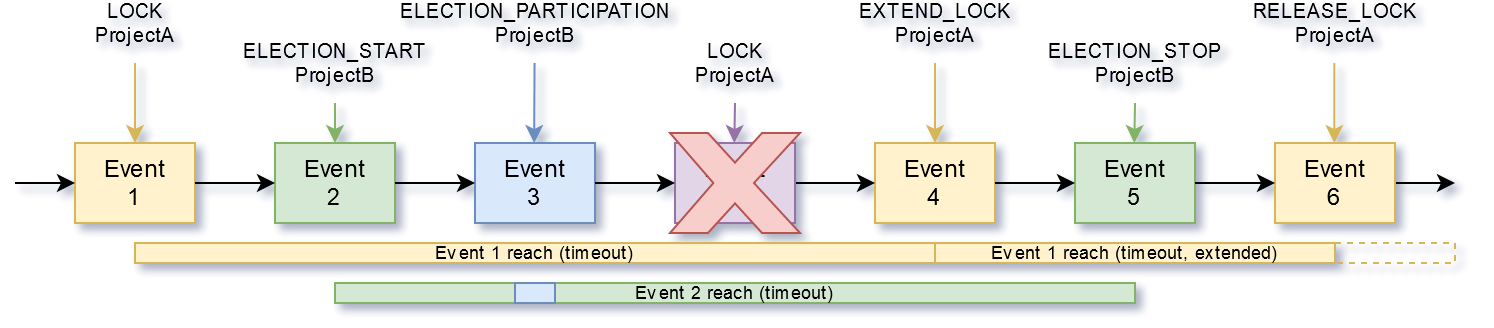
\includegraphics[width=0.9\textwidth]{events.png}
	\label{winslow:com:events}
	\caption{Sample event and lock series with lifetimes}
\end{figure}

\section{Backend Driver}

Docker REST API vs 
\todo{ Nomad} \autoref{analysis:layer_3}



\section{Execution Management}

As noted in \autoref{analysis:layer_1}, the central business logic is to deciding when and issuing stage executions.
There are two general approaches in doing so, both will be discussed next.

\subsection{Remote Execution}

In this approach, the job is executed on a remote machine and not on the same node which has the responsibility in managing the execution.
Continuous Integration (CI) platform Jenkins\cite{jenkins:main} as well as GitLab\cite{gitlab:main} do offer this approach.
The so called slave node (Jenkins) or runner (GitLab) is accessed by the CI through a common interface (SSH in these cases) to start the job execution.
Jenkins and GitLab even copy a custom binary onto the slave node, that is then managing the execution on the remote machine locally.
This is due to the complexity in executing the job for a given configuration as well as being able to continue the execution on disconnects or maintenance reboots of the master machine.

In this scenario, the CI instance requires and stores login credentials for every remote machine to be able to login whenever needed.
The system administrator therefore has to create a new user account on the remote machine, install required programs and environments (bot Jenkins and GitLab require an JRE\footnote{Java Runtime Environment}).
In case of an security breach on the CI instance, the attacker is also able to login on all remote nodes and execute arbitrary programs as well \todo{there is probably a great article about an issue like this!?}.

\todo{WRONG, on GitLab YOU need to intall/setup the runner}

GitLab follows another approach, the system administrator has to manually install the GitLab Runner\footnote{\todo{cite}} on a slave node and is then able to add this runner to a Project.
The security risk is somewhat similar to Jenkins: once an attacker has access to the CI instance, arbitrary code can be uploaded and executed on the remote machines. \todo{but no ssh login .... until first binary uploaded}

\todo{winslow is more secure because of docker and therefore limited access to the system, no network..?}

\subsection{Local Execution}

Executing a job locally means running a job on the same machine as the program that is monitoring the execution.
This has the advantage of having all libraries, tools and resources already present \todo{and is without the threat of connection loss to the remote machine}.
But in the case of Jenkins and GitLab, this is means, each CI instance is separate from the others.
There is no integration between those instance in this configuration.
What is missing Jenkins and GitLab here is the capability to decentralize their core task of managing projects, resources and executions.

\todo{scheduling}


\subsection{The approach for Winslow}

\todo{.}

potentially many executions -> easier when local

need watch hardware utilization closely

enables-ish \enquote{spin up a new instance and you are ready to go} slogan



\section{Backend Nomad}

\todo{.}

\section{Large File Storage organization}

\subsection{Stage storage}


Thinking about the storage organisation for the pipeline and its stages, a few expectations and concerns arise.
First of all, to redo a stage, one needs to be able to access the files that were the result of one, two or multiple stages before the current.
Sometimes a stage wants to access intermediate data produces by multiple previous stages.
Next, the input video footage needs to be accessed by multiple stages throughout the pipeline execution.
Finally, some stage results are not intermediate but final results.
\todo{examples}

The first and second concern can be solved by providing a workspace directory for each stage, that is copied from the logically previous stage.
Once the computation of a stage is completed, the workspace is considered immutable and only used to source new workspaces from.
This works fine for small intermediate results, but it does not work very well for large files - like the video footage.
Starting a new stage will take as long as the copy of multiple gigabytes on a spinning devices take (\todo{sample GB and time}), require unnecessary storage due to multiple copies and provides no benefits in an archival and version control sense, because the video footage is not altered.
So there needs to be another storage pool for input data, that is globally accessible and never changed: the global input storage pool.
Providing one further storage pool for final results (global output pool), concern number three and four are also solved.

Because the very first stage has no workspace to source its files from, on creation of the pipeline a workspace directory for the \enquote{zeroths} stage is created.
The user can then provide the very first stage with a predefined and non-empty workspace if necessary.

Because in the implementation of this project NFS was used, this also solves one further problem that was experienced in the prototyping phase: copying files on NFS (and many other network filesystems like Samba) is a client operation.
This means, the client reads the input file and writes to the output file.
Because the common network used (gigabit in this case) is slower than spinning disk sequential read/writes (network: 112 Megabytes/s in theory, divided by two because read+write on the same connection: 56 Megabytes/s, spinning enterprise disk: about 170 Megabytes/s \todo{test on johnny5}), this operation does not only take unnecessary long but also renders the network connection close to unusable for any other participant in the network that needs to use parts of the same physical route.

To ensure that the global input and the previous intermediate results are not altered, the Docker daemon is instructed to mounted them as read-only filesystems.
This makes it impossible\footnote{When there is no bug in the implementation of mount or Docker} for the stage to accidently delete or alter the wrong files\footnote{Like in this scenario, where an unexpected space in a script caued people to loose their home directory: \todo{steam rm -rf incident}}.


\begin{figure}[H]
	\centering
	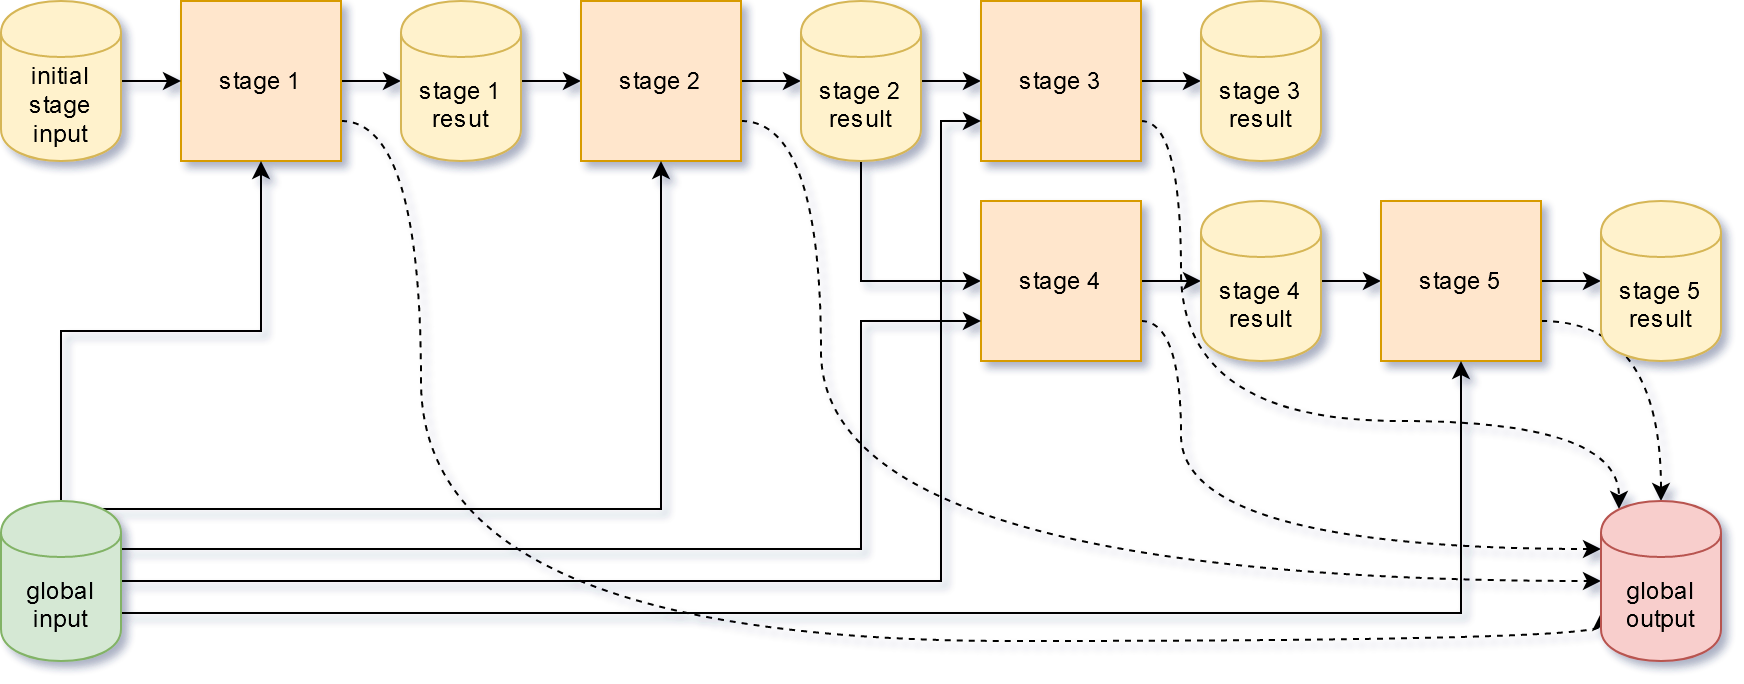
\includegraphics[width=0.9\textwidth]{stage-storage.png}
\end{figure}

In summary, the storage pool solution looks like this:

\todo{check paths}
\begin{itemize}
	\item \monospaceinline{/input} is mounted read-only from \\ \monospaceinline{nfs-server:/winslow/workspaces/<pipeline-id>/input}
	\item \monospaceinline{/output} is mounted with write permissions from \\ \monospaceinline{nfs-server:/winslow/workspaces/<pipeline-id>/output}
	\item \monospaceinline{/workspace} is mounted with write permissions from \\ \monospaceinline{nfs-server:/winslow/workspaces/<pipeline-id>/<stage-id>} \\
	and was created by the copying the workspace directory of the logically previous stage
\end{itemize}

\todo{define logically previous stage -> previous stage on linear execution and ... when jumping around}



initial input

stage execution does not need to depend on the result of the exact previous



\section{Job Scheduling / Election System}
\label{design:election}
\label{election:affinity_and_aversion} \todo{.}

\todo{affinity}
\todo{aversion}

Utilizing Event Bus for timely limited elections and to ensure that there are no concurrent election for a single project.

\todo{what about concurrent elections on multiple projects}

\todo{regarding locking: check for updatable, try to lock, check for updatable again, update, unlock}

\todo{on unlock: check updatable}



\todo{scheduling / job assignment/pull strategy}

\todo{graph displaying over time lock and election}

\section{CPU RAM Network IO Monitoring}

\section{User Interface}

\todo{REST request, read only: no lock; for changes: POST -> LOCK -> update -> RELEASE, on RELEASE Winslow gets notified and checks whether the new configuration leads to a new stage execution}

\section{File system}

\todo{docker can auto mount nfs to container}

\subsection{Every node has a connection to every other node}

\subsection{Centralized broker}

\subsection{Tree hierarchy}

\subsection{outcome}




\section{Communication and Node Management}

The system that shall be developed, is supposed to spread jobs onto execution nodes as available.
There are two main approaches in nod management and job assignment.



\subsection{Centralized Management, Remote Execution}

In the central management approach, there is always exactly one leader at any given moment in time.
It is the responsibility of this leader to decide what to execute and where to execute it.

\subsection{Decentralized Management, Local Execution}

\subsection{Combinations worth noting}

stupid:
 - centralized management, local execution
 - decentralized management, remote execution
 
combination, decentralized + some remote slaves

\subsection{Architecture}

event based

common file system for communication because minimum requirements

stick to unix principles(list): simple, human readable intermediate format

voting/election by capabilities and 'will' of a node to run a stage

\todo{providing live hw utilization}

\todo{the whole properties thingy}

\subsection{Failure handling}
\todo{handling failed stages}

\todo{handling failed nodes}

\section{Communication/Event architecture?}

\section{Targeting capabilities}

\subsection{General thoughts}

\section{Planned}

\section{Implementation details}

\section{Synchronization, Locking, publishing events}

\section{REST for UI}



\subsection{Atomicy of (Unix) Filesystems}

\subsection{Atomicy and behavior of NFS in particular}

\subsection{Using as lock backend}

\subsection{Using as election backend}




\section{Agile development}


\section{Continuous Deployment}

Ironically, although mentioned as unusable in \autoref{.}\todo{.} for the use case Winslow wants to fulfil, it will use GitLab CI for continuous \todo{delivery} of runnable Docker Images.
Every code change in the Git repository will trigger a new build pipeline, that builds and tests Winslow, packages all dependencies \todo{nomad} into a Docker image and pushes it to our in house private Docker Registry \todo{.}.
The \todo{execution nodes} will pull the latest image whenever they restart or are triggered to restart.
\todo.